\documentclass[11pt,a4paper]{article}
\usepackage[margin=2.6cm]{geometry}
\usepackage{amsmath,amssymb}
\usepackage{booktabs,array}
\usepackage{enumitem}
\usepackage{xcolor}
\usepackage{tikz}
\usepackage{pgfplots}
\pgfplotsset{compat=1.17}
\usepackage[colorlinks=true,linkcolor=teal!70!black,citecolor=teal!70!black,urlcolor=teal!70!black]{hyperref}

\definecolor{bandA}{HTML}{008A7C}
\definecolor{bandB}{HTML}{C2610C}
\newcommand{\tagbox}[2]{\textsf{\scriptsize\colorbox{#1!12}{\textcolor{#1!70!black}{#2}}}}
\newcommand{\est}{\tagbox{gray}{established}}
\newcommand{\lit}{\tagbox{blue}{literature}}
\newcommand{\ours}{\tagbox{orange}{ours}}
\newcommand{\lP}{\ell_{\mathrm P}}

\title{Is It Spacetime?\\[4pt]
\large Discrete universes measured by counting: a manifold detector, a first particle,\\ and the memory a growing universe needs}
\author{Draft v5 --- internal notebook checkpoint}
\date{27 October 2026\\[2pt]\small Not for circulation. Claims are tagged \est, \lit{} or \ours.}

\begin{document}
\maketitle

\begin{abstract}
We model spacetime as a discrete set of events with a causal order and nothing else, and ask which ways of producing such universes give something that looks like spacetime, and what a growing universe has to remember. (1) Lorentz-invariant discreteness gives every event one neighbour per unit of rapidity, a known result. We take the finite size of the universe as the physical cutoff ($\eta_{\max}\approx142$, cosmological frame); with a finite past it leaves no trace in Sorkin's $1+1$ d'Alembertian. (2) A counting toolkit in $1+1$: proper time from the longest chain, an exact rectangle identity $d^2=2V_AV_B/V_C$ for causal-overlap distances, curvature from how that estimate drifts with depth ($1-R\tau^2/16$), and a Lorentzian embedding that works as a manifold detector from $N\approx100$--$200$. (3) Applying it: grown universes fail; $e^{-\beta S}$ universes pass in the continuum phase and fail in the layered phase, and at $N=400$ the two phases show hysteresis over $0.08\le\beta\le0.7$; quantum weights $e^{i\beta S}$ suppress few-layer universes, but at reachable $\beta$ only through the spread of the action. Quantum growth with one amplitude per birth is covariant without normalization; whether its past stabilises (the ``future factor'' test) is open. (4) A first actor: Johnston's sum over chains. In a random 2D order its average is exactly $\tfrac12L_n(\mu/2)$ (Laguerre) at interval size $n$, whose Poisson average is Johnston's $\tfrac12J_0(m\tau)$; continuum-like universes pass, crystals and grown universes fail. (5) Memory. Each birth needs only a few past events, but they span the whole age. Per de Sitter patch the memory is finite but a spacetime-volume law in $d=2$--$4$ ($\sim10^{244}$ events in $3+1$ against a horizon entropy of $\sim10^{122}$). Coarse cells do not capture what a newborn feels. In exact quantum sums, phases do not reduce the memory; relative to what events can see, they turn alternatives into records. Gravity in $3+1$ and interactions are still absent.
\end{abstract}

\section{The question and the rules}
In 1900 Planck assumed that energy comes in discrete quanta. We ask the analogous question for spacetime: can it be a discrete set of events that only \emph{looks} continuous from far away, with general relativity (GR) as its large-scale description? The working constraints are:
\begin{enumerate}[label=\textbf{C\arabic*},leftmargin=*,itemsep=1pt]
\item \textbf{Discrete spacetime.} Events and the causal order between them; the continuum is a large-scale limit.
\item \textbf{No background.} No absolute space and no fixed aether; every statement is about relations between events.
\item \textbf{Non-locality regulated by the finite size of the universe} (Sec.~\ref{sec:cutoff}).
\item \textbf{Local Lorentz invariance} for all boosts well below the cutoff.
\item \textbf{A cosmological clock computed from the universe's own state}, e.g.\ the longest chain back to the beginning. It may be used as a bookkeeping clock for growth, but local laws must not depend on it, and predictions must not depend on which relational clock is used. Its frame should coincide with the matter (CMB) frame \est; that is a test, not an input.
\item \textbf{Newton and Einstein from far away.}
\item \textbf{Creation (and perhaps destruction) of events drives expansion}, possibly through quantum creation operators.
\item \textbf{The links between events are quantum.}
\end{enumerate}
Missing so far is \emph{matter}: nothing in the model yet plays the role of what gravitates.

A \emph{fixed background} is structure the laws refer to but which nothing affects; C2 forbids it. A \emph{dynamical preferred-frame field}, such as the Einstein-aether~\cite{JacobsonMattingly01}, breaks local Lorentz invariance. A \emph{preferred frame of the state}, such as the CMB frame, comes from the contents of the universe while the laws stay invariant. C5 allows only the last kind.

\paragraph{The storyline.} Section~\ref{sec:cutoff} explains why the finite size of the universe is our regulator. A discrete universe is only useful if it looks like spacetime, so Sec.~\ref{sec:toolkit} builds tools that answer ``is it spacetime?'' from the order alone, Sec.~\ref{sec:which} applies them to classical growth, $e^{-\beta S}$ weights and quantum weights and growth, Sec.~\ref{sec:matter} puts a first particle on the order, and Sec.~\ref{sec:film} asks how much of the past a growing universe must remember, classically and quantum mechanically.

\section{Neighbours and the cosmological cutoff}\label{sec:cutoff}
\paragraph{One neighbour per unit of rapidity.} \lit{} Following causal set theory~\cite{BLMS87,Surya19}, $y$ is a \emph{neighbour} (a \emph{link}) of $x$ if $y$ is in the causal future of $x$ and no other event lies causally between them. In $1+1$ dimensions, with density $\rho$, write a future event as $u=t-x=\tau e^{-\eta}$, $v=t+x=\tau e^{\eta}$, where $\tau$ is the proper time from the origin and $\eta$ the rapidity. The area element is $dt\,dx=\tau\,d\tau\,d\eta$, and the interval up to the event has area $\tau^2/2$, so it is empty with probability $e^{-\rho\tau^2/2}$. Therefore
\begin{equation}
\langle N_{\rm links}\rangle=\int d\eta\int_0^\infty \rho\,\tau\,e^{-\rho\tau^2/2}\,d\tau=\int d\eta\cdot 1 .
\label{eq:onepereta}
\end{equation}
There is one expected neighbour per unit of rapidity, so an infinite universe gives every event infinitely many neighbours. This is the elementary core of the Bombelli--Henson--Sorkin theorem~\cite{BHS06}: Lorentz-invariant discreteness is non-local~\cite{Sorkin07}.

\paragraph{A finite universe caps the rapidity.} \ours{} A neighbour at proper time $\tau$ and rapidity $\eta$ lies at distance $r\approx(\tau/2)e^{\eta}$. In a universe of size $L$ this cannot exceed $L$, so
\begin{equation}
\eta_{\max}\simeq\ln\frac{2L}{\lP}\approx142,
\end{equation}
with $L\approx4.4\times10^{26}$\,m and $\lP=1.6\times10^{-35}$\,m. Lorentz kinematics has been tested up to $\eta\approx25$--$27$ (GZK protons and the highest-energy cosmic rays~\cite{CG99}), far below the cutoff. The only frame singled out is that of the universe as a whole, a frame of the state, as C5 requires. In $1+1$ dimensions an event has about $2\eta_{\max}\approx280$ future neighbours. In $3+1$ dimensions the cutoff leaves $\sim(L/\lP)^2\approx10^{124}$ (Appendix~\ref{app:dropped} lists the numerology we avoid).

\paragraph{Does the cutoff show up in wave propagation?} \lit{} Sorkin's $1+1$ d'Alembertian~\cite{Sorkin07} acts on a field by summing it over the past of $x$ with layer weights. For density $\rho=\ell^{-2}=1$ and averaged over sprinklings,
\begin{equation}
\bar B\phi(x)=4\Big[-\tfrac12\phi(x)+\int_{J^-(x)}\!d^2y\;e^{-V}\big(1-2V+\tfrac12V^2\big)\phi(y)\Big],
\label{eq:box}
\end{equation}
where $V$ is the volume of the interval between $y$ and $x$. The three terms are links, next-to-links and next-to-next-to-links with weights $1,-2,1$. On a plane wave $\phi=e^{-i(pu+qv)}$ it gives $4pq$, which is $\Box\phi/\phi$ in the convention used here (checked numerically).

\ours{} The kernel integrates to \emph{zero} per unit rapidity, $\int_0^\infty\tau\,d\tau\,e^{-\tau^2/2}(1-\tau^2+\tau^4/8)=0$, but there are infinitely many units of rapidity. The integral in Eq.~\eqref{eq:box} is therefore only conditionally convergent: when $\phi$ does not oscillate along one light-cone direction, the answer depends on how the far past is cut off. We compared two cut-offs in the cosmological frame.
\begin{enumerate}[leftmargin=*,itemsep=1pt]
\item \emph{A rapidity wedge}, $|\eta|\le\eta_{\max}$, with $\tau$ integrated to infinity. Write the past event as $(u,v)=-(\tau e^{-\eta},\tau e^{\eta})$. Then $s=pe^{-\eta}+qe^{\eta}$ is the phase per unit $\tau$, and the bracket becomes $-\tfrac12+\int d\eta\,h(s)$, with $h$ the $\tau$-integral of the kernel times $e^{is\tau}$.
\item \emph{A finite past region}, the diamond $0\le a\le U$, $0\le b\le U$ of displacements along $u$ and $v$ ($U\simeq L$). This is what a universe of finite age provides. The $b$-integral is elementary (incomplete gamma functions), and $a$ is integrated numerically.
\end{enumerate}
For a constant field, the diamond gives the bracket in closed form: $-\tfrac12+\tfrac12\big[1-(1-A)e^{-A}\big]$ with $A=U^2/2$, i.e.\ zero up to $e^{-A}$. The ``$\tfrac12$'' is assembled at the two null edges of the region, $\tfrac14$ each; the inner integral over the edge region reduces to digamma values, $-\tfrac12\int_0^\infty e^{-x}(1-2x+\tfrac12x^2)\ln x\,dx=\tfrac14$. The results:
\begin{center}\small
\begin{tabular}{@{}lccc@{}}
\toprule
field & wedge & finite past & $\Box$\\
\midrule
constant & $-2$ & $0$ & $0$\\
exact null wave ($p=0$) & $-1$ & $0$ & $0$\\
massive, $pq=10^{-9}$, a light-cone wavelength $>L$ ($L=e^{10}$) & $-0.6$ to $-1.8$ & $4pq$ & $4pq$\\
\bottomrule
\end{tabular}
\end{center}
With an oscillating field the missing $\tfrac14$ per null direction comes from the interior, at $u\sim1/p$; with a non-oscillating one it comes from the edge of the past. The wedge has no edge, so it loses it. Aslanbeigi, Saravani and Sorkin~\cite{ASS14} define the plane-wave eigenvalue only where the integral converges absolutely (complex momenta with a timelike, future-pointing imaginary part) and reach real momenta as a limit. Their $1+1$ result, $g(Z)=-Ze^{Z/2}E_2(Z/2)$ with $Z=p\cdot p/\rho$, goes smoothly to zero at null momentum, in agreement with the finite past.

\emph{Consequence.} In $1+1$ the finite size of the universe leaves Sorkin's $\Box$ exactly continuum-like, up to $e^{-(\text{past volume})}$, for every wavelength. Through this operator the cutoff produces no dispersion correction and no change in the speed of light. That is good news for C3 and C4, which do not conflict here, and bad news for predictions. The $3+1$ case is not done.

\section{Geometry by counting}\label{sec:toolkit}
Everything in this section uses only the causal order. To test the tools we generate universes by Poisson sprinkling at density $\rho$ into a known spacetime, discard the coordinates, and compare what the tools find with the truth. We write $\ell=\rho^{-1/2}$ for the discreteness length in $1+1$ dimensions: a patch of volume $\ell^2$ holds one event on average.

\subsection{Time: the longest chain}
\lit{} The proper time between two events is estimated by the longest chain between them~\cite{BrightwellGregory91}. In a sprinkled $1+1$ diamond this is the longest increasing subsequence of a random permutation, with mean $\simeq2\sqrt n$ and Tracy--Widom fluctuations $\simeq0.90\,n^{1/6}$~\cite{BDJ99}, so $\delta\tau/\tau\simeq0.45\,n^{-1/3}$. Our simulations reproduce both (\texttt{sims/causal\_diamond.py}). Equivalently $\tau^2=2V$, where the volume $V$ of the interval is its number of events divided by $\rho$. \ours{} (interpretation) Geometry measured by counting is intrinsically fuzzy. The fuzziness is a relation between events, not a smearing in a background space.

\subsection{Space: causal overlaps and a rectangle identity}
\lit{} For two events $a,b$ with neither before the other, Boguñá and Krioukov~\cite{BK24} pick an event $c$ in their common past and compare the intervals $I(c,a)$ and $I(c,b)$:
\begin{equation}
A=I(c,a)\setminus I(c,b),\quad B=I(c,b)\setminus I(c,a),\quad C=I(c,a)\cap I(c,b),\qquad O=\frac{V_C}{\min(V_A,V_B)+V_C}.
\end{equation}
With $c$ chosen at equal proper time $\tau_c$ from $a$ and $b$, in $1+1$ dimensions $d=\tau_c(1-O)/\sqrt O$. We re-derived this.

\begin{figure}[t]
\centering
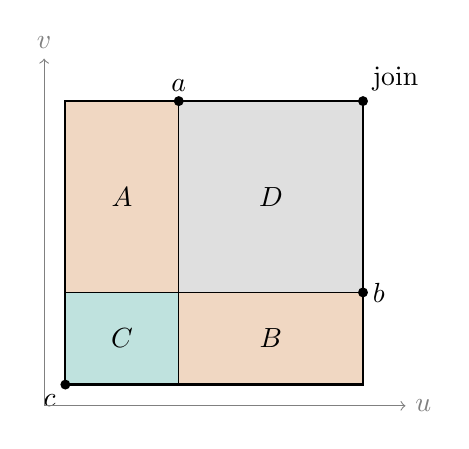
\begin{tikzpicture}[scale=0.9]
  \fill[bandA!25] (0,0) rectangle (1.6,1.3);
  \fill[bandB!25] (0,1.3) rectangle (1.6,4);
  \fill[bandB!25] (1.6,0) rectangle (4.2,1.3);
  \fill[gray!25] (1.6,1.3) rectangle (4.2,4);
  \draw[thick] (0,0) rectangle (4.2,4);
  \draw (1.6,0) -- (1.6,4); \draw (0,1.3) -- (4.2,1.3);
  \node at (0.8,0.65) {$C$}; \node at (0.8,2.65) {$A$}; \node at (2.9,0.65) {$B$}; \node at (2.9,2.65) {$D$};
  \fill (0,0) circle (2pt) node[below left] {$c$};
  \fill (1.6,4) circle (2pt) node[above] {$a$};
  \fill (4.2,1.3) circle (2pt) node[right] {$b$};
  \fill (4.2,4) circle (2pt) node[above right] {join};
  \draw[->,gray] (-0.3,-0.3) -- (4.8,-0.3) node[right] {$u$};
  \draw[->,gray] (-0.3,-0.3) -- (-0.3,4.6) node[above] {$v$};
\end{tikzpicture}
\caption{The rectangle identity in light-cone coordinates (rotate by $45^\circ$ for the usual picture). The rectangle from $c$ to the join of $a$ and $b$ splits into four tiles: the overlap $C$, the strips $A$ and $B$ seen by only one of $a,b$, and the diamond $D$ with $a$ and $b$ at its corners. Opposite tiles have equal products, $C\cdot D=A\cdot B$, and $D$ encodes the distance between $a$ and $b$.}
\label{fig:tiles}
\end{figure}

\ours{} In $1+1$ dimensions the choice of $c$ does not matter. Step by step (Fig.~\ref{fig:tiles}):
\begin{enumerate}[leftmargin=*,itemsep=1pt]
\item In light-cone coordinates $dt\,dx=du\,dv/2$, and for spacelike events $d^2=\Delta x^2-\Delta t^2=-\Delta u\,\Delta v$.
\item With $c$ at the origin, $I(c,a)=[0,u_a]\times[0,v_a]$ and $I(c,b)=[0,u_b]\times[0,v_b]$ are rectangles. Take $u_a<u_b$, $v_a>v_b$.
\item The rectangle from $c$ to the join $(u_b,v_a)$ splits into $C=[0,u_a]\times[0,v_b]$, $A=[0,u_a]\times[v_b,v_a]$, $B=[u_a,u_b]\times[0,v_b]$ and $D=[u_a,u_b]\times[v_b,v_a]$.
\item Opposite tiles have equal products: $C\cdot D=u_av_b\,\Delta u\,\Delta v=A\cdot B$.
\item $D$ has $(u,v)$-area $|\Delta u\,\Delta v|=d^2$, hence volume $d^2/2$.
\end{enumerate}
Therefore, for \emph{any} $c$ in the common past,
\begin{equation}
d^2=\frac{2\,V_AV_B}{V_C}\;\approx\;\frac{2\,N_AN_B}{\rho\,(N_C+1)} .
\label{eq:rect}
\end{equation}
The strips $A$ and $B$ are long and thin, so they hold many events even when $d\sim\ell$; this is also why the Boguñá--Krioukov estimator works at short distances. Their equal-time choice is the special case $V_A=V_B$. The identity holds only in $1+1$ dimensions, because in more dimensions the overlap of two diamonds is not a diamond. The counts $N_A,N_B,N_C$ come from disjoint regions and are therefore independent Poisson variables. $N_AN_B$ is then unbiased, but $1/N_C$ is not; $1/(N_C+1)$ has mean $(1-e^{-\lambda})/\lambda$ and removes the bias. Before this fix, a flat control read $+11\%$.

\begin{table}[t]
\centering\small
\begin{tabular}{@{}rccc@{}}
\toprule
$N$ & $d<2\ell$ & $2\ell$--$10\ell$ & $>10\ell$\\
\midrule
1000 & 23\% & 6.5\% & 5.2\%\\
2000 & 15\% & 5.0\% & 3.4\%\\
4000 & 19\% & 5.1\% & 2.5\%\\
\bottomrule
\end{tabular}
\caption{Median relative error of Eq.~\eqref{eq:rect} with the deepest $c$, flat $1+1$ sprinklings, 4 seeds (\texttt{sims/s4a\_overlap\_distance.py}). There is no significant bias above $2\ell$. The large-distance error falls roughly as $N^{-1/2}$. Below $2\ell$ the error stays at $\sim20\%$: this is the discreteness scale.}
\label{tab:dist}
\end{table}

\subsection{Curvature: the estimate drifts with depth}
\lit{} Curvature can be read from counts through the Benincasa--Dowker operator~\cite{BD10,DowkerGlaser13}. In our runs (session 2) it gave the right sign and order of magnitude for de Sitter, but was noisy at $10^4$ events. Related continuum results give the curvature corrections to the volume of a small causal diamond~\cite{GibbonsSolodukhin07} and to chain counts inside it~\cite{RSS13}.

\ours{} The rectangle identity provides a second route. Two-dimensional de Sitter space, $ds^2=(H\eta)^{-2}(-d\eta^2+dx^2)$, has the same light cones as flat space, so $A,B,C,D$ are the same rectangles, but volumes are weighted by $dV=2\,du\,dv/(H^2(u+v)^2)$. Integrating over a rectangle gives a logarithm of the conformal times at its corners,
\begin{equation}
V_\square=\frac{2}{H^2}\ln\frac{\eta_L\,\eta_R}{\eta_{\rm bottom}\,\eta_{\rm top}},
\end{equation}
and $C\cdot D=A\cdot B$ no longer holds exactly. For $a,b$ on one slice and $c$ a proper time $\tau_c$ below them, expanding for small $d$ and then small $\tau_c$ gives
\begin{equation}
\frac{d_{\rm est}^2}{d^2}=1-\frac{(H\tau_c)^2}{8}+\dots=1-\frac{R\,\tau_c^2}{16}+\dots,\qquad R=2H^2 .
\label{eq:drift}
\end{equation}
In flat space every $c$ gives the same answer. In curved space the answer depends on how deep $c$ lies, and the size of that drift is the curvature. We checked the coefficient $1/8$ numerically from the exact volumes (0.1252 at small $\tau$). In sprinklings ($\rho=10^4$, test events inserted by hand $14\ell$ apart), the measured ratio agrees with the continuum in every depth bin for 200 fresh seeds, and a flat control shows no drift. Fitting $d_{\rm est}^2=\alpha+\beta\tau^2$ with $\tau$ also from counts gives $R=-16\beta/\alpha$:
\begin{center}\small
\begin{tabular}{@{}rcc@{}}
\toprule
$\rho$ & flat (true $R=0$) & de Sitter (true $R=2$; continuum fit in this window $2.13$)\\
\midrule
4000 & $-0.7\pm0.6$ & $1.3\pm0.7$\\
$10^4$ & $0.3\pm0.4$ & $1.6\pm0.4$\\
\bottomrule
\end{tabular}
\end{center}
It is right on average, but a single pair is useless: the run-to-run spread is about 4, so about 100 pairs are needed for $\pm0.4$. Three web searches found no curvature version of the overlap estimator, so it is \ours{} in the sense ``not found in a brief search''.

\subsection{Shape: an embedding that doubles as a manifold detector}
\lit{} Given squared intervals between $M$ events, classical multidimensional scaling (MDS) with a Lorentzian Gram matrix reconstructs coordinates (cf.~\cite{Johnston25}). With $s_{ij}=(x_i-x_j)^T\eta(x_i-x_j)$, double centring $G=-\tfrac12JSJ$, $J=I-\mathbf 1\mathbf 1^T/M$, gives $G=X\eta X^T$. A $1+1$ Lorentzian set shows one large negative eigenvalue (time) and one large positive one (space), with the rest near zero, and the eigenvectors give coordinates up to a Lorentz transformation.

\ours{} With $s=-2N(I)/\rho$ for timelike pairs and Eq.~\eqref{eq:rect} for spacelike pairs (all from counts), on $M=150$ events of a flat sprinkling ($N=2000$):
\begin{itemize}[leftmargin=*,itemsep=1pt]
\item positions are recovered to $0.43\pm0.07\,\ell$ across a region about $38\ell$ wide, better than one event spacing;
\item the map to the true coordinates is a Lorentz transformation to within 3--10\%;
\item the spectrum is $\lambda_-\approx-2.2$, $\lambda_+\approx2.2$, with all others below $0.1$;
\item a $2+1$ sprinkling fed through the same $1+1$ pipeline shows \emph{two} large positive eigenvalues: the spectrum counts spatial dimensions even with the wrong distance formula.
\end{itemize}
We turn this into a detector with four intrinsic numbers: $w_2$, the share of the spectrum in one time and one space direction; $r_\pm$, the ratio of the second to the first eigenvalue of each sign; and the \emph{stress}, the rms misfit of the best $1+1$ Minkowski embedding. Two calibrations matter. (i) Size: on flat universes, stress and $r_+$ are $0.22/0.42$ at $N=20$, $0.33/0.41$ at $50$, $0.20/0.16$ at $100$, $0.11/0.08$ at $200$ and $0.08/0.05$ at $400$. The detector is reliable only from $N\approx100$--$200$; below $50$ a flat universe looks like a crystal. (ii) Curvature: on de Sitter diamonds of fixed $N=400$, the stress stays at the flat value up to $H\tau\approx1$ and rises to $0.21$ at $H\tau=4$. So the embedding answers ``is it a sheet?'', while Eq.~\eqref{eq:drift} measures curvature.

\section{Which universes are spacetime?}\label{sec:which}
\subsection{Classical growth fails}
\lit{} In sequential growth~\cite{RideoutSorkin00} events are born one at a time, and each newborn picks causes among existing events. \ours{} We ran two rules: fixed link probability $p$ (a steady state of fixed width) and $p_n=3/n$ (an expanding universe from a single first event; layers of $1,2,3,3,5,7,\dots,\sim280$ events). The second rule uses the birth order as a hidden clock, which C2 forbids; the covariant route is through cosmological renormalisation of $p$~\cite{MORS01,AhmedRideout10}. Neither rule gives a $1+1$ spacetime. Their Myrheim--Meyer dimension drifts with scale, falling to $\sim1.2$ for fixed $p$ (a thin tube) and rising from $1.6$ to $2.8$ for $p=3/n$. On the detector at $N=100$ they fail every number: $w_2\approx0.33$ against $0.65$ for the calibration, and stress $\approx0.65$ against $0.19$.

\subsection{Weights $e^{-\beta S}$: a continuum phase and a crystal}
\lit{} Weighting $1+1$ orders by $e^{-\beta S}$, with $S$ the Benincasa--Dowker action, gives a phase transition between a continuum-like phase and a layered ``crystal''~\cite{Surya12,BHS08,GOS18}. \ours{} We reproduce it ($\beta_c\approx1.2,0.7,0.5$ for $N=30,50,70$, at non-locality parameter $\epsilon=0.21$). An $O(N^2)$ Metropolis update (a swap changes only two rows and columns of the causal matrix, so $K'=CC+C'E+EC$ with thin $E$) brings $N=200$ to $0.03$\,s per sweep. Two clocks, height and past volume, give the same cosmic ordering in both phases, except for pairs within one or two layers (C5).
\begin{center}\small
\begin{tabular}{@{}lccccc@{}}
\toprule
$N=200$ & ordering fraction & layers & $w_2$ & $r_+$ & stress\\
\midrule
flat calibration & 0.50 & 24 & 0.75 & 0.07 & 0.10\\
$\beta=0.05$ (continuum) & 0.51 & 24 & 0.74 & 0.10 & 0.11\\
$\beta=0.6$ (crystal) & 0.59 & 9 & 0.82 & \textbf{0.39} & \textbf{0.28}\\
\bottomrule
\end{tabular}
\end{center}
The continuum phase is indistinguishable from flat spacetime. The crystal asks for an extra spatial direction and fits badly.

\paragraph{$N=400$: hysteresis.} \ours{} At $N=400$ we start each chain either hot (a random order) or cold (a two-layer order, the lowest-action layered state we found): 80 chains of $1.5\times10^4$ sweeps on the cluster (tasks that hit the time limit are read from checkpoints and logs). Hot and cold chains never meet for $0.08\le\beta\le0.7$. Cold crystals melt only at $\beta\le0.05$; hot chains leave the continuum only at $\beta\ge0.45$ and then stick in a $\sim10$-layer state. So the transition is only bracketed, $0.05<\beta_c(400)<0.45$. The cold crystal thins as $\beta$ grows (5, 3, 2 layers at $\beta=0.08$, $0.12$, $\ge0.2$), and the two-layer order has far lower action than anything the hot chains reach ($S/N\approx-34$ against $-12$), so it is very likely the large-$\beta$ ground state and the $N=200$ ``crystal'' above a metastable intermediate. Locating $\beta_c$ needs a method that crosses the barrier, such as parallel tempering.

\subsection{Quantum weights $e^{i\beta S}$}
\paragraph{Records.} \ours{} (lesson from session 2) Phases only matter if different histories end in the same outcome. If every universe is its own outcome, $|e^{i\beta S}|^2=1$ and nothing interferes. We therefore choose a \emph{record}, a relational property shared by many universes, and let universes with the same record interfere: $P_q(r)=|A_r|^2/\sum_{r'}|A_{r'}|^2$, $A_r=\sum_{\text{record }r}e^{i\beta S}$.

\paragraph{A bound.} \ours{} (likely known) Since $|e^{i\beta S}|=1$, $|A_r|$ is at most the number of universes with record $r$. In the quantum sum, rare universes such as crystals can only win if the common, manifold-like ones cancel each other out. With $e^{-\beta S}$, rare universes with low action win by sheer weight.

\paragraph{Exact sums, $N\le9$.} \ours{} Summing over all $N!$ orders with record = number of layers, $e^{-\beta S}$ collapses onto flat layered universes ($N=9$, $\beta=8$: 2 layers with 76\%), while $e^{i\beta S}$ suppresses them by destructive interference (2 layers: 0\%; 5 layers: 62\%). Such universes are too small to say whether they are spacetime.

\paragraph{Sampling, $N=200$.} \ours{} The amplitude of a record is proportional to the average of $e^{i\beta S}\mathbf 1_r$ over uniformly random orders, which can be sampled. This works while the average phase, $\approx e^{-\beta^2\sigma_S^2/2}$, is not tiny. At $N=200$, $\sigma_S=12.0$, so the average phase is $0.49$ at $\beta=0.1$ and $0.06$ at $\beta=0.2$. We drew $10^6$ orders on the cluster (50 independent seeds; errors are jackknife over seeds). The record is the layer count (the height clock of C5), grouped into bins. The probability of the few-layer bin ($\le22$ layers; the mean is $24.6$), relative to its value at $\beta=0$:
\begin{center}
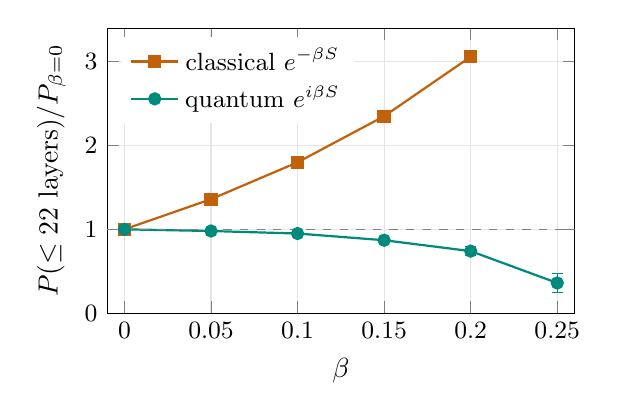
\begin{tikzpicture}
\begin{axis}[width=0.62\textwidth,height=5.2cm,xlabel={$\beta$},ylabel={$P(\le22\ \mathrm{layers})/P_{\beta=0}$},xtick={0,0.05,0.1,0.15,0.2,0.25},xticklabel style={/pgf/number format/fixed,/pgf/number format/precision=2},
  legend pos=north west,legend style={font=\small,draw=none},grid=major,grid style={gray!20},tick label style={font=\small},
  ymin=0,ymax=3.4,xmin=-0.01,xmax=0.26]
\addplot[thick,bandB,mark=square*] coordinates {(0,1)(0.05,1.36)(0.1,1.80)(0.15,2.35)(0.2,3.06)};
\addlegendentry{classical $e^{-\beta S}$}
\addplot[thick,bandA,mark=*,error bars/.cd,y dir=both,y explicit] coordinates {(0,1)+-(0,0.005)(0.05,0.98)+-(0,0.005)(0.1,0.95)+-(0,0.005)(0.15,0.87)+-(0,0.02)(0.2,0.74)+-(0,0.05)(0.25,0.36)+-(0,0.11)};
\addlegendentry{quantum $e^{i\beta S}$}
\addplot[dashed,gray] coordinates {(-0.01,1)(0.26,1)};
\end{axis}
\end{tikzpicture}
\end{center}
Classically, raising $\beta$ drives the universe toward few layers, the approach to the crystal. Quantum weights do the opposite and suppress few-layer universes. This agrees with the exact sums and with Loomis and Carlip~\cite{LoomisCarlip18}, who show analytically that $e^{iS}$ suppresses two-layer orders. (The classical reweighting is reliable up to $\beta=0.2$, with an effective sample size of 1{,}022.)

\emph{But the mechanism is simple.} Within each record the action is close to Gaussian, with spread $\sigma_r$. Then $|A_r|\approx n_r e^{-\beta^2\sigma_r^2/2}$, so
\begin{equation}
P_q(r)\propto n_r^2\,e^{-\beta^2\sigma_r^2},
\end{equation}
and this reproduces the sampled numbers to $0.001$ for $\beta\le0.15$. Few-layer universes have a slightly larger spread ($\sigma=11.73$ against $11.48$), so their phases cancel more. In the range that sampling can reach, ``quantum suppression'' is a variance effect, not a structured interference pattern. With record = stress quartile, quantum and classical weights drift by the same small amount (Q1: $0.261\pm0.003$ against $0.258$ at $\beta=0.15$). A $1{,}600$-sample pilot that suggested a large shift toward manifold-like universes was noise. Uniform sampling is exhausted at $\beta\approx0.2$ for $N=200$; real interference structure needs exact or layer-by-layer methods.

\subsection{Quantum growth, one event at a time}
\lit{} In sequential growth every causal set can be grown by adding events one at a time, each newborn taking any down-set of the existing events as its past~\cite{RideoutSorkin00}. \ours{} A birth $f$ changes the Benincasa--Dowker action by
\begin{equation}
\Delta S_f = 4\epsilon - 8\epsilon^2\sum_{x<f} f(n_{xf},\epsilon),
\label{eq:dS}
\end{equation}
with $n_{xf}$ the number of events between $x$ and $f$ (summing over births reproduces $S$ to $10^{-10}$). Give each birth the amplitude $e^{i\beta\Delta S_f}$. The amplitude of a causal set $C$ is then (number of natural labellings of $C$)$\,\times e^{i\beta S(C)}$: covariant, with the counting measure supplied by the growth itself. Summed exactly to $N=8$ ($2.8\times10^6$ growth paths): at $\beta=0$ a three-layer, Kleitman--Rothschild-like sector carries $80\%$ of the weight; a window $\beta\epsilon^2\approx0.3$ suppresses it by interference, as known~\cite{LoomisCarlip18}, but what is left is not yet spacetime-like.

\paragraph{No normalization; does the past stabilise?} \ours{} Classical growth normalizes the transition weights at every step. Doing the same with amplitudes breaks covariance, and the violation grows with $N$ (a factor of $\sim10$ at $N=22$). We drop it and instead ask that the past stabilise as the universe grows. For a grown stem $X$ define the \emph{future factor}
\begin{equation}
F_N(X)=\sum_{\text{continuations }X\to N}e^{i\beta(S_N-S_X)} .
\end{equation}
The probabilities of questions about the past settle as $N\to\infty$ only if the ratios $F_N(X)/F_N(Y)$ converge: the future must factorize. Memoizing unlabelled posets gives exact $F_N$ to $N=10$. At $\beta=0$ the ratio of the two 2-element stems is exactly $3/(N+1)\to0$ (the layered sector wins). Inside the window that ratio locks its phase near $\pi$ by $N\approx8$--$10$ (drift $\sim10\%$), while 3-element stems still move by $20$--$50\%$. Inconclusive; $N=11$ is running on the cluster. As far as our search went, nobody computes $F_N$: growth models built with a sum rule~\cite{SuryaZalel20} make $F_N=1$ by construction. Stems are the right observables, since stem sets generate the covariant questions classically~\cite{BDGHS03}.

\section{A first actor: a particle as a sum over chains}\label{sec:matter}
An event of the model is an atom of spacetime volume, about a Planck 4-volume, not a laboratory event: a femtometre-scale collision spans $\sim10^{79}$ of them. Particles have to live \emph{on} the events. \lit{} A classical free particle maximises proper time, so it is the longest chain~\cite{BrightwellGregory91}. Johnston's quantum particle~\cite{Johnston08} sums over all chains, with amplitude $a$ per hop and $b$ per stop: with $\Phi=aC$ ($C$ the causal matrix),
\begin{equation}
K=\Phi+b\Phi^2+b^2\Phi^3+\dots=\Phi(I-b\Phi)^{-1},\qquad a=\tfrac12,\ b=-m^2/\rho\ \ (1+1).
\end{equation}
Step by step: in $1+1$ the expected number of chains $x\prec z_1\prec\dots\prec z_k\prec y$ in an interval of area $\tau^2/2$ is $(\rho\tau^2/2)^k/(k!)^2$, so $\langle K\rangle=\tfrac12\sum_k(-(m\tau/2)^2)^k/(k!)^2=\tfrac12J_0(m\tau)$, the retarded Klein--Gordon propagator. We reproduce it on sprinklings.

\paragraph{An exact target from the order alone.} \ours{} $K$ depends only on $\mu=m^2/\rho$: $K(x,y)=\tfrac12\sum_kc_k(x,y)(-\mu/2)^k$, with $c_k$ the number of $k$-element chains inside the interval. In a uniformly random 2D order, the $n$ events of an interval are again a random 2D order, and $k$ of them form a chain with probability $1/k!$, so $E[c_k\,|\,n]=\binom nk/k!$~\cite{Pinsky06} and
\begin{equation}
E[K\,|\,n]=\tfrac12\sum_k\binom nk\frac{(-\mu/2)^k}{k!}=\tfrac12L_n(\mu/2)\;\approx\;\tfrac12e^{\mu/4}J_0\!\big(\sqrt{2\mu(n+\tfrac12)}\big),
\end{equation}
a Laguerre polynomial in the interval size. Averaging over Poisson $n$ with mean $\rho\tau^2/2$ gives exactly $\tfrac12J_0(m\tau)$, so Johnston's result is the Poisson average of this one, which needs no density at all. The pieces are textbook; the assembled statement was not found in 13 causal-set papers searched in full text (INSPIRE not searched). Expanding in $\mu$, the first order that can fail is the ordering fraction, i.e.\ the Myrheim--Meyer dimension: the propagator is a resummed tower of dimension tests.

\paragraph{Tests.} \ours{} Continuum-like $N=400$ universes match the target as well as random controls do (rms $0.013$--$0.020$ at $\mu=0.05$). Crystals fail: a 4-layer one has no interval larger than 9 events, so $K$ never turns negative and ``mass'' means nothing; a 7-layer one falls far below the target (too many chains). All classically grown universes ($N=1500$) fail systematically, and one ($p=0.02$) runs away to $|K|\approx10$, twenty times the 2D bound $\tfrac12$. In curved 2D a term $(R\tau^2/48)J_2(m\tau)$ appears~\cite{NXDS17}, a candidate curvature probe at fixed $n$. Limits: one scalar, retarded propagator only, no backreaction, and an exact target only in 2D. Interactions are open: Johnston considered summing vertices over events and set it aside as ambiguous.

\section{How much past does the present need?}\label{sec:film}
A cosmological clock (C5) suggests rewriting the sum over histories as a film: a state for ``now'' and an operator taking it to the next moment (C7). That needs the action to split into steps that each see only a small piece of the past. We measured how far that goes.

\paragraph{Thick height layers fail.} \ours{} Truncate $S$ to pairs at most $m$ height layers apart. Links skip layers: in continuum $1+1$ orders, $61\%$ of links skip at least one layer at $N=200$, and the longest spans 23 of about 24 layers. To keep the error below $0.25\,\sigma_S$ the memory must be $m\approx9,10,\gtrsim14$ layers at $N=100,200,400$, about $40\%$ of the age. At $N\le9$ the truncated quantum sums deviate from the exact ones by up to 0.47 (total variation) when only $4.5\%$ of the pairs are dropped. A volume clock gives different answers from the height clock, so a height truncation also breaks C5. (The crystal needs only $m\approx4$.)

\paragraph{Growth and causal closeness.} \lit{} We let events be born one at a time, each with any set of existing events as its past but never in the past of an existing event: Rideout--Sorkin's internal temporality~\cite{RideoutSorkin00}. Every causal set can be grown this way, the dates (heights) of events never change, and $e^{i\beta S}$ does not depend on the birth order. \ours{} In the birth step~\eqref{eq:dS}, keeping only $x$ with $n_{xf}\le10$ leaves an error of $0.06$--$0.07\,\sigma_S$ at $N=100,200,400$, flat in $N$, and $0.07$ in the crystal. The cut is a count, so it uses no clock. About $16,22,29$ past events are kept per birth, growing like $\ln N$, but they span the whole age: the influence of the past is sparse and long-range in time, and local in ``events in between''.

\paragraph{The thick present.} \ours{} If $f$ needs $x$, it also needs everything between them, so a state holding all events that some later birth still needs is self-contained. We measured its size in hindsight, which gives a lower bound:
\begin{center}\small
\begin{tabular}{@{}ll@{}}
\toprule
universe ($1+1$, $n_{\rm cut}=10$) & state\\
\midrule
diamond (open space) & $0.6$--$0.8\,N$\\
static circle of length $W$ & $\approx0.5\,W^2$, independent of the age\\
decelerating closed FRW ($a\propto t^{1/2}$) & oldest needed event $\approx0.5\,W$ of conformal time back\\
accelerating closed FRW ($e^{Ht}$, $t^2$) & $0.9$--$1.0$ of the past, never retired\\
\bottomrule
\end{tabular}
\end{center}
An event stays needed until its light cone wraps around space, about $W/2$ of conformal time. The film therefore has a finite memory if and only if the universe has no event horizon. Our universe accelerates, so by this measure its present needs the whole past. The per-birth step is cheap; the storage is not.

\paragraph{Per observer: finite, but a volume law.} \ours{} The ``whole past'' of an accelerating universe is a stack of de Sitter static patches. Per patch, the events still needed are finite and stationary, so the horizon does bound the memory. But they scale with the spacetime volume: about $3\rho$, $6.3\rho$, $9.6\rho$ events in $d=2,3,4$, with $\rho=1/(\ell H)^d$ from 25 to 400 (exponent $\approx0.97$; an area law would give $0$, $\tfrac13$, $\tfrac12$). The reason is Little's law from queueing: memory $=$ birth rate $\times$ how long each event stays needed. The second factor, $1$--$3$ Hubble times, does not depend on $\rho$, because under C4 an event cannot be forgotten until its light cone leaves the patch. In $3+1$ with $\ell\approx\lP$ this is $\sim(L_H/\lP)^4\approx10^{244}$ events per patch, against a de Sitter entropy of $\sim10^{122}$ (a comparison of scales, not a match). Either the count overstates what the universe must hold (a clumsy description of a simpler state), or the dynamics is missing something.

\paragraph{A ladder.} \ours{} Three levels of description, each needing less memory:
\begin{center}\small
\begin{tabular}{@{}l>{\raggedright}p{0.36\textwidth}l>{\raggedright\arraybackslash}p{0.2\textwidth}@{}}
\toprule
level & the future needs & memory scales as & status\\
\midrule
events & the past events newborns can link to & spacetime volume & measured (above)\\
geometry and fields & data on one slice (an initial-value problem) & spatial volume & \est{} for GR; open for us\\
area & slice data minus what gravity forbids & horizon area & needs gravity\\
\bottomrule
\end{tabular}
\end{center}
Coarse-graining into cells of a fixed size $\xi$ keeps a volume law with a smaller coefficient. An area law in $3+1$ would need $(L/\xi)^4=(L/\ell)^2$, i.e.\ $\xi=\sqrt{L\ell}$, a cell growing with the universe. This is the UV/IR scale of Cohen, Kaplan and Nelson~\cite{CKN99}, near the dark-energy length; we note it and do not lean on it (any combination of $L$ and $\lP$ is a power of $10^{61}$).

\paragraph{The second rung fails for the causal-set operator.} \ours{} Put a test event at the top of a flat $1+1$ diamond and compute what it feels: Sorkin's operator on $\phi=1$, raw and smeared ($\epsilon=0.1$, $0.03$)~\cite{Sorkin07}. Then shuffle the events inside each cell of a light-cone grid, keeping the count per cell, and recompute. The share of the variance created by shuffling, $f_{\rm micro}=E[\mathrm{Var}(b\,|\,\text{cells})]/\mathrm{Var}(b)$, is 1 if the cell counts explain nothing and 0 if they suffice (means $\approx0$ in all runs; 16--24 independent bases):
\begin{center}\small
\begin{tabular}{@{}lcc@{}}
\toprule
events per cell & raw ($N=500/2000/8000$) & smeared $\epsilon=0.03$ ($N=500/2000/8000$)\\
\midrule
$\ge31$ & $1.0/1.0/1.0$ & $1.0/0.90/0.99$\\
2 & $0.99/1.07/0.95$ & $0.20/0.30/0.66$\\
0.5 & $0.92/0.94/$-- & $0.07/0.12/$--\\
\bottomrule
\end{tabular}
\end{center}
The raw operator has no macrostate at all: moving events within cells holding half an event already scrambles it. The smeared one admits one only at $\lesssim2$ events per cell, and that gets worse as the universe grows (cells tilted by a boost are worse still). What a newborn feels comes from a thin sliver along its light cone that stretches over the whole past, which no fixed cell resolves. Classical coarse-graining compresses by at most a small factor. Caveats: one newborn, flat space, cells tied to one frame.

\paragraph{Quantum memory as a matrix.} \ours{} Let $p$ be the universe after $k$ births (unlabelled) and $F$ the final universe, and let $B_{pF}$ be the sum of $e^{i\beta\Delta S}$ over all growths from $p$ to $F$; its row sums are the future factors $F_N$. Pasts with equal rows can share a classical memory slot, so the classical memory is $\log_2$ of the number of distinct rows; linearly dependent rows can share quantum memory, so the quantum memory is $\log_2\mathrm{rank}\,B$ (the bond dimension of a sequentially generated state~\cite{Schon05}; quantum models can need less memory than classical ones~\cite{Gu12}). A structural fact follows from Eq.~\eqref{eq:dS}: $\Delta S$ depends only on the endpoints, so $B=\mathrm{diag}(e^{-i\beta S_p})\,\mathrm{Count}\,\mathrm{diag}(e^{i\beta S_F})$, and \emph{the phases cannot change any memory measure} when the outcome is the whole final universe. They can only matter for coarser outcomes. With a coarse record of $F$ (height, minimal and maximal events, links; $N=7$, $k=5$, 63 pasts) the effective memory (entropy of normalized singular values) is $3.78$ bits at $\beta=0$, $4.05$ at $\beta=7$, $4.45$ at $\beta=12$ and $5.34$ for random phases: interference adds memory.

\paragraph{Records.} \ours{} One motivation (Roberto's) is that links might stay undetermined precisely because nothing stores them, with quantum mechanics as the universe's way of saving memory. Ideas deriving quantum theory from limited information exist~\cite{Zeilinger99,Spekkens07}; a brief search found none deriving it from a storage limit of the universe. Two corrections sharpen it: storing a probability distribution or a wavefunction costs more than storing one state, so any saving must come from \emph{summing} over what is never determined; and the saving needs one real history, since a universe holding all branches stores more, not less. We adopt Sorkin's quantum measure theory~\cite{Sorkin94}: unchanged dynamics, one real history, and probabilities only for alternatives that no longer interfere. A record is then an alternative that can never interfere again, which needs no threshold, unlike physical collapse models, which need a rate: relativistic GRW~\cite{Tumulka06}, or gravity-related Di\'osi--Penrose collapse, whose parameter-free form is excluded~\cite{Donadi20}. Two findings. (i) If every event saw its whole past, everything inside any future event's past would be a record and the memory a volume law again; any saving needs events that see their past only partially. (ii) Taking as the screen what the last-born event sees (its full past, its size and number of links, or only the number of links), with the universe after $k$ births as the alternatives, the mean coherence between alternatives at $N=8$, $k=5$ is:
\begin{center}\small
\begin{tabular}{@{}lccc@{}}
\toprule
screen & $\beta=0$ & $\beta=8$ & random phases\\
\midrule
full past & 0.55 & 0.21 & 0.15\\
size, links & 0.75 & 0.38 & 0.22\\
links & 0.97 & 0.72 & 0.49\\
\bottomrule
\end{tabular}
\end{center}
No pair is ever exactly decohered. The coarser the screen, the more stays undetermined; that saving is classical ($\beta=0$ has no interference). The phases make alternatives \emph{more} distinguishable: here quantum mechanics makes records rather than saving memory. Caveats: $N\le8$, alternatives labelled by birth order rather than covariant stems, one observer.

\section{Discussion}
\paragraph{Where this sits.} The kinematics is causal set theory: links, infinite valency, Number $=$ Volume, the longest chain as proper time, growth, the Benincasa--Dowker action, the phase transition and the overlap distances are theirs. Our additions are (i) the finite size of the universe as the regulator of the non-locality, with the cosmological frame accepted as a frame of the state; (ii) the rectangle identity~\eqref{eq:rect}; (iii) curvature from the depth drift~\eqref{eq:drift}; (iv) a calibrated, intrinsic manifold detector; (v) quantum record probabilities by sampling at $N=200$, with the $|A_r|$ bound and the variance formula $P_q\propto n_r^2e^{-\beta^2\sigma_r^2}$; and (vi) the check that a finite past keeps Sorkin's $\Box$ exact in $1+1$. Items (ii)--(iv) were not found in brief searches. (v) confirms a known trend at larger $N$ and explains it. (vi) agrees with the analytic treatment of~\cite{ASS14}; what we add is the finite universe as the physical regulator. (vii) The causal-closeness cut of the growth step and the thick-present rule (memory $\approx W/2$ of conformal time; finite iff no event horizon) were not looked for in the literature beyond Rideout--Sorkin's growth rule, so they are \ours{} in the weakest sense: not searched. (viii) The Laguerre form of Johnston's propagator at fixed interval size: built from known pieces, not found assembled. (ix) The future-factor criterion and its exact computation; no paper computes it. (x) The memory results of Sec.~\ref{sec:film}: the volume law per patch, the failure of cell coarse-graining, and the endpoint-phase theorem for $B$; not searched beyond causal-set entanglement entropy, which also shows a volume law without truncation~\cite{SorkinYazdi18}. On the dynamics side, a cosmological clock (C5) would license writing the sum over histories as a transfer matrix between cosmic-time layers, with operators that create events (C7). That puts us next to causal dynamical triangulations and Hořava--Lifshitz gravity, whose preferred foliation is fundamental rather than emergent; we must show that the difference is real.

\paragraph{Limitations.}
\begin{enumerate}[leftmargin=*,itemsep=1pt]
\item \emph{Everything is $1+1$.} The rectangle identity is $1+1$ only, and $1+1$ GR has no Newtonian limit, so C6 needs $3+1$.
\item \emph{$3+1$ is not tamed}: $10^{124}$ neighbours per event.
\item \emph{Matter is a probe, not a source.} One free scalar on a fixed order; no interactions, no backreaction, nothing gravitates.
\item \emph{Small universes.} The detector needs $N\gtrsim100$--$200$. Exact quantum sums stop at $N\approx12$, and sampled ones are limited by the average phase.
\item \emph{The quantum result is a variance effect.} Sampling reaches only $\beta\lesssim0.2$ at $N=200$. The record and $\epsilon$ are chosen, not derived.
\item \emph{No prediction.} In $1+1$ the cutoff is invisible to wave propagation, not merely far beyond tests.
\item \emph{Memory.} Per patch it is a volume law. Neither cell coarse-graining nor quantum phases reduce it in what we computed; whether quantum states with records do at large $N$ is open. Exact quantum sums stop at $N\approx11$ and use birth-order alternatives, not covariant stems.
\end{enumerate}

\paragraph{Next steps.}
\begin{itemize}[leftmargin=*,itemsep=1pt]
\item The future factor at $N=11$ (running): does the past stabilise inside the window?
\item Records with covariant alternatives (stems) and events that see a fixed budget of their past; count records per patch against births.
\item The $J_2$ curvature probe at fixed interval size, and the propagator on universes near the transition.
\item Locate $\beta_c(400)$ with parallel tempering.
\item The cutoff check, the overlap estimator and the detector in $2+1$ and $3+1$.
\end{itemize}

\appendix
\section{Paths explored and dropped}\label{app:dropped}
\begin{itemize}[leftmargin=*,itemsep=1pt]
\item \textbf{A regular crystal of events.} Polygonal light cones and a lattice rest frame~\cite{Burago,Weyl}.
\item \textbf{Quantum blur of positions.} Blur in \emph{what}? It presupposes a background, and an equal superposition over rapidity cannot be normalised.
\item \textbf{A quantum chain as the source of blur.} Background-dependent. The atomic-linewidth analogy was overstated: coupling \emph{reduces} the blur.
\item \textbf{Expansion as a source and gravity as a sink of points} (river model~\cite{HamiltonLisle08}). It needs an aether.
\item \textbf{A link to Bell non-locality.} Links are timelike; Bell correlations are spacelike.
\item \textbf{$(L/\lP)^2\sim10^{122}$ and the cosmological constant.} Numerology: every combination of $L$ and $\lP$ is a power of $10^{61}$.
\item \textbf{The manifold detector on exact quantum sums.} At $N\le12$ the detector cannot tell a flat universe from a crystal; replaced by sampling.
\item \textbf{$\eta_{\max}$ as a dispersion correction.} Killed in $1+1$ (Sec.~\ref{sec:cutoff}). An intermediate version claimed a jump to $-1/\ell^2$ once a wavelength exceeds $L$; that was an artefact of a rapidity-wedge regulator.
\item \textbf{$\eta_{\max}$ as the long-link suppression of Caravelli and Markopoulou~\cite{CM12}.} A different object: a spatial lattice with external time, giving an energy-dependent mass.
\item \textbf{A transfer matrix on thick height layers.} The memory must grow to $\sim40\%$ of the age, and the truncation breaks clock independence (Sec.~\ref{sec:film}).
\item \textbf{A finite-state film in an accelerating universe.} The thick present never retires its events (Sec.~\ref{sec:film}).
\item \textbf{Quantum weights at $N=100$ on stress quartiles.} Superseded by $N=200$; the small-sample hint was noise.
\item \textbf{Normalizing quantum growth at every step.} Breaks covariance, increasingly with $N$.
\item \textbf{``Memory shared with the outside'' as the area-law part of the memory.} It is all of it: outside events need old events forever.
\item \textbf{A cell macrostate for what a newborn feels} (the second rung of the ladder). Shuffling within cells scrambles it, worse as $N$ grows.
\item \textbf{``Probabilities are cheaper to store than states.''} The opposite; only summing over undetermined alternatives can save memory.
\item \textbf{Di\'osi--Penrose collapse with the discreteness length as its size cut-off.} A smaller size means faster collapse; excluded by the underground bound.
\item \textbf{Exactly orthogonal futures of birth-order pasts as records.} With an open future no record ever forms: any two small pasts fit in a common future.
\end{itemize}

\begin{thebibliography}{99}\small
\bibitem{JacobsonMattingly01} T.~Jacobson, D.~Mattingly, ``Gravity with a dynamical preferred frame'', Phys.\ Rev.\ D 64, 024028 (2001), gr-qc/0007031.
\bibitem{BLMS87} L.~Bombelli, J.~Lee, D.~Meyer, R.~D.~Sorkin, ``Space-time as a causal set'', Phys.\ Rev.\ Lett.\ 59, 521 (1987).
\bibitem{Surya19} S.~Surya, ``The causal set approach to quantum gravity'', Living Rev.\ Rel.\ (2019), arXiv:1903.11544.
\bibitem{BHS06} L.~Bombelli, J.~Henson, R.~D.~Sorkin, ``Discreteness without symmetry breaking: a theorem'', gr-qc/0605006.
\bibitem{Sorkin07} R.~D.~Sorkin, ``Does locality fail at intermediate length-scales?'', gr-qc/0703099.
\bibitem{CG99} S.~Coleman, S.~L.~Glashow, ``High-energy tests of Lorentz invariance'', Phys.\ Rev.\ D 59, 116008 (1999), hep-ph/9812418.
\bibitem{BrightwellGregory91} G.~Brightwell, R.~Gregory, ``Structure of random discrete spacetime'', Phys.\ Rev.\ Lett.\ 66, 260 (1991).
\bibitem{BDJ99} J.~Baik, P.~Deift, K.~Johansson, ``On the distribution of the length of the longest increasing subsequence of random permutations'', J.\ Amer.\ Math.\ Soc.\ 12, 1119 (1999).
\bibitem{BK24} M.~Boguñá, D.~Krioukov, ``Measuring spatial distances in causal sets via causal overlaps'', Phys.\ Rev.\ D 110, 024008 (2024), arXiv:2401.17376.
\bibitem{BD10} D.~M.~T.~Benincasa, F.~Dowker, ``The scalar curvature of a causal set'', Phys.\ Rev.\ Lett.\ 104, 181301 (2010).
\bibitem{DowkerGlaser13} F.~Dowker, L.~Glaser, ``Causal set d'Alembertians for various dimensions'', arXiv:1305.2588.
\bibitem{GibbonsSolodukhin07} G.~W.~Gibbons, S.~N.~Solodukhin, ``The geometry of small causal diamonds'', Phys.\ Lett.\ B 649, 317 (2007), hep-th/0703098.
\bibitem{RSS13} M.~Roy, D.~Sinha, S.~Surya, ``The discrete geometry of a small causal diamond'', Phys.\ Rev.\ D 87, 044046 (2013), arXiv:1212.0631.
\bibitem{Johnston25} S.~Johnston, ``Simpler embeddings of causal sets into Minkowski spacetime'', arXiv:2502.09701.
\bibitem{RideoutSorkin00} D.~P.~Rideout, R.~D.~Sorkin, ``A classical sequential growth dynamics for causal sets'', Phys.\ Rev.\ D 61, 024002 (2000).
\bibitem{MORS01} X.~Mart\'in, D.~O'Connor, D.~P.~Rideout, R.~D.~Sorkin, ``On the renormalization transformations induced by cycles of expansion and contraction in causal set cosmology'', Phys.\ Rev.\ D 63, 084026 (2001).
\bibitem{AhmedRideout10} M.~Ahmed, D.~Rideout, ``Indications of de Sitter spacetime from classical sequential growth dynamics of causal sets'', Phys.\ Rev.\ D 81, 083528 (2010).
\bibitem{Surya12} S.~Surya, ``Evidence for a phase transition in 2D causal set quantum gravity'', arXiv:1110.6244.
\bibitem{BHS08} G.~Brightwell, J.~Henson, S.~Surya, ``A 2D model of causal set quantum gravity: the emergence of the continuum'', arXiv:0706.0375.
\bibitem{GOS18} L.~Glaser, D.~O'Connor, S.~Surya, ``Finite size scaling in 2d causal set quantum gravity'', Class.\ Quant.\ Grav.\ (2018), arXiv:1706.06432.
\bibitem{Burago} D.~Burago, ``Periodic metrics''; statement in arXiv:1104.4460.
\bibitem{Weyl} H.~Weyl, \emph{Philosophy of Mathematics and Natural Science} (1949).
\bibitem{ASS14} S.~Aslanbeigi, M.~Saravani, R.~D.~Sorkin, ``Generalized causal set d'Alembertians'', JHEP 06 (2014) 024, arXiv:1403.1622.
\bibitem{LoomisCarlip18} S.~P.~Loomis, S.~Carlip, ``Suppression of non-manifold-like sets in the causal set path integral'', arXiv:1709.00064.
\bibitem{CM12} F.~Caravelli, F.~Markopoulou, ``Disordered locality and Lorentz dispersion relations'', Phys.\ Rev.\ D 86, 024019 (2012), arXiv:1201.3206.
\bibitem{Lloyd02} S.~Lloyd, ``Computational capacity of the universe'', Phys.\ Rev.\ Lett.\ 88, 237901 (2002), quant-ph/0110141.
\bibitem{Johnston08} S.~Johnston, ``Particle propagators on discrete spacetime'', Class.\ Quant.\ Grav.\ 25, 202001 (2008), arXiv:0806.3083.
\bibitem{Pinsky06} R.~G.~Pinsky, ``Law of large numbers for increasing subsequences of random permutations'', arXiv:math/0407353, eq.~(1.1).
\bibitem{NXDS17} Nomaan~X, F.~Dowker, S.~Surya, ``Scalar field Green functions on causal sets'', Class.\ Quant.\ Grav.\ 34, 124002 (2017), arXiv:1701.07212.
\bibitem{SuryaZalel20} S.~Surya, S.~Zalel, ``A criterion for covariance in complex sequential growth models'', arXiv:2003.11311.
\bibitem{BDGHS03} G.~Brightwell, H.~F.~Dowker, R.~S.~Garc\'ia, J.~Henson, R.~D.~Sorkin, ``\,`Observables' in causal set cosmology'', Phys.\ Rev.\ D 67, 084031 (2003), gr-qc/0210061.
\bibitem{SorkinYazdi18} R.~D.~Sorkin, Y.~K.~Yazdi, ``Entanglement entropy in causal set theory'', Class.\ Quant.\ Grav.\ 35, 074004 (2018), arXiv:1611.10281.
\bibitem{CKN99} A.~G.~Cohen, D.~B.~Kaplan, A.~E.~Nelson, ``Effective field theory, black holes, and the cosmological constant'', Phys.\ Rev.\ Lett.\ (1999), hep-th/9803132.
\bibitem{Schon05} C.~Sch\"on, E.~Solano, F.~Verstraete, J.~I.~Cirac, M.~M.~Wolf, ``Sequential generation of entangled multiqubit states'', Phys.\ Rev.\ Lett.\ 95, 110503 (2005), quant-ph/0501096.
\bibitem{Gu12} M.~Gu, K.~Wiesner, E.~Rieper, V.~Vedral, ``Quantum mechanics can reduce the complexity of classical models'', Nature Commun.\ 3, 762 (2012), arXiv:1102.1994.
\bibitem{Zeilinger99} A.~Zeilinger, ``A foundational principle for quantum mechanics'', Found.\ Phys.\ 29, 631 (1999).
\bibitem{Spekkens07} R.~W.~Spekkens, ``Evidence for the epistemic view of quantum states: a toy theory'', Phys.\ Rev.\ A 75, 032110 (2007).
\bibitem{Sorkin94} R.~D.~Sorkin, ``Quantum mechanics as quantum measure theory'', Mod.\ Phys.\ Lett.\ A 9, 3119 (1994), gr-qc/9401003.
\bibitem{Tumulka06} R.~Tumulka, ``A relativistic version of the Ghirardi--Rimini--Weber model'', J.\ Stat.\ Phys.\ 125, 821 (2006), quant-ph/0406094.
\bibitem{Donadi20} S.~Donadi, K.~Piscicchia, C.~Curceanu, L.~Di\'osi, M.~Laubenstein, A.~Bassi, ``Underground test of gravity-related wave function collapse'', Nature Phys., arXiv:2111.13490.
\bibitem{HamiltonLisle08} A.~J.~S.~Hamilton, J.~P.~Lisle, ``The river model of black holes'', Am.\ J.\ Phys.\ 76, 519 (2008).
\end{thebibliography}
\end{document}
